\section{Requisitos de Software}

\subsection{Web e Mobile}

Para os requisitos a seguir, o termo "aplicação" é usado para designar tanto aplicativo móvel quanto aplicação web.

\textbf{1. A aplicação deve exibir os dados capturados pelos sensores}

Os dados coletados pelos sensores instalados na estufa devem ser transmitidos às aplicações web e mobile, de forma que possam ser apresentados ao proprietário da estufa em tempo real.

\textbf{2. A aplicação deve permitir ajuste de temperatura do sistema.}

Como cada hortaliça necessita de temperatura específica, é importante poder alterar a temperatura dentro da estufa para que a hortaliça tenha um crescimento desejável.

\textbf{3. A aplicação deve permitir a troca de água do sistema.}

Embora a troca de água seja acionada automaticamente quando o nível de pH esteja fora da faixa aceitável, o usuário deve ser capaz de acionar esta funcionalidade manualmente.

\textbf{4. A aplicação deve exibir notificações quando o nível de pH da água estiver abaixo ou acima do nível ideal.}

Como um nível impróprio de pH da água é prejudicial para hortaliças, a aplicação deve exibir uma notificação sempre que, por algum motivo, o nível de pH fique acima ou abaixo do especificado como ideal. 

\textbf{5. A aplicação deve exibir notificações quando a temperatura estiver abaixo ou acima do nível ideal.}

A estufa deve ser mantida em uma faixa de temperatura especificada como ideal para as hortaliças. Sempre que, por algum motivo, a temperatura interna da estufa fique acima ou abaixo desta faixa, uma notificação deve ser exibida pela aplicação.

\textbf{6. A aplicação deve exibir opções com configurações pré-definidas para cultivo.}

Para facilitar a utilização da estufa por pessoas que não possuem conhecimentos prévios sobre cultivo de hortaliças, a aplicação deve possuir um banco de dados populado com informações sobre as condições ideais de cultivo das variedades mais comuns de hortaliças.


\section{Web Service}

A solução exige componentes capaz de manter comunicação unificada entre a estufa e as interfaces web e mobile. A necessidade de se atualizar parâmetros em tempo real orienta ao uso de uma solução com rabbitmq juntamente com o protocolo de comunicação AMQP.

A API que será desenvolvida terá auxílio do microframework Falskm, tendo este a responsabilidade pela integração entre os componentes de software. A solução da API seguirá o padrão arquitetural de microsserviços. 

\section{Linguagens e frameworks}

A construção do backend será desenvolvida em Python com o auxílio do framework Nameko, sendo este desenvolvido especialmente para aplicações de microsserviços. Além disso, será utilizado o microframework Flask para a implantação da API e a geração de rotas para requisição de páginas via AMQP, para que seja possível a conversão dos dados coletados em formatos em JSON, sendo este subsídio de entrada o frontend.

Para o frontend, serão utilizados o ReactJS para a aplicação web e o React Native na aplicação mobile. 

\section{Sistema mobile de controle}

A estufa poderá ser controlada via um aplicativo instalado no smartphone do proprietário da mesma. Isto será alcançado por meio de uma comunicação com o WebService citado acima.

Por meio do aplicativo, o proprietário poderá monitorar e alterar as condições internas da estufa de forma remota. Os dados coletados por meio dos sensores instalados no interior da estufa serão transmitidos ao smartphone do proprietário em tempo real. Quaisquer alterações definidas pelo aplicativo irão acionar os componentes relevantes para efetivar as mesmas.

O aplicativo mobile será desenvolvido utilizando o framework React Native. Esta tecnologia foi selecionada pois ela permite uma comunicação facilitada com o WebService definido acima.

\section{Sistema Web de Controle}

O sistema web oferece uma alternativa para o controle de estufa. Será desenvolvida em React JS, também se conectará ao WebService e oferecerá os mesmos mecanismos de controle disponíveis no Sistema Mobile de Controle.

\section{Histórias de Usuário}

Seguindo as recomendações do SCRUM, uma metodologia ágil de desenvolvimento de software, foram definidas histórias de usuário que representam funcionalidades planejadas do sistema. Cada história foi analisada pela equipe de desenvolvimento e pontuada segundo seu nível de complexidade. A seguir encontra-se a listagem delas.

\textbf{US01 - Visualizar medições}

\textbf{Pontuação:} 3

\textbf{Eu como:} Usuário

\textbf{Desejo:} visualizar as medições feitas pelos sensores

\textbf{Para que:} possa ter um monitoramento sobre a hortaliça plantada

\begin{itemize}
	\item Exibir valores atuais de temperatura, potencial hidrogeniônico, nível de água, consumo de água, luminosidade.
	\item Exibir valores históricos
		\subitem Gráficos de linha
		\subitem Exibir dados referentes ao dia, semana, mês, ano
		\subitem Utilizar cores diferentes para cada grandeza
\end{itemize}

\textbf{US02 - Login de usuário}

\textbf{Pontuação:} 5

\textbf{Eu como:} Usuário

\textbf{Desejo:} logar no sistema

\textbf{Para que:} tenha acesso a modificações no ambiente interno da estufa.

\begin{itemize}
	\item Exibir tela de login.
	\item Utilizar endereço de email para login.
	\item Utilizar PIN para autenticação
		\subitem PIN de 4 dígitos
\end{itemize}

\textbf{US03 - Cadastro de usuário}

\textbf{Pontuação:} 3

\textbf{Eu como:} Usuário

\textbf{Desejo:} me cadastrar no sistema

\textbf{Para que:} ganhe acesso autenticado ao sistema.

\begin{itemize}
	\item Utilizar número de série para cadastro inicial pelo aplicativo.
	\item Cadastrar endereço de e-mail como login.
	\subitem Enviar confirmação de cadastro como e-mail
	\item Cadastrar PIN para autenticação
	\subitem PIN de 4 dígitos
\end{itemize}

\textbf{US04 - Manter hortaliças}

\textbf{Pontuação:} 3

\textbf{Eu como:} Usuário

\textbf{Desejo:} manter uma hortaliça no banco de dados

\textbf{Para que:} diferentes tipos de hortaliças possam ser mantidos de forma automatizada pela estufa

\begin{itemize}
	\item Cadastrar uma nova hortaliça.
		\subitem Temperatura
		\subitem Luminosidade
		\subitem Nome
		\subitem Tempo de cultivo
	\item Excluir uma hortaliça
	\subitem Exibir confirmação de exclusão
	\item Cadastrar PIN para autenticação
	\subitem PIN de 4 dígitos
	\item Editar uma hortaliça
	\subitem Visualizar uma hortaliça
\end{itemize}

\textbf{US05 - Alertar usuário}

\textbf{Pontuação:} 2

\textbf{Eu como:} Sistema

\textbf{Desejo:} alertar o usuário sobre mudanças no ambiente interno da estufa

\textbf{Para que:} ele possa fazer as alterações necessárias

\begin{itemize}
	\item Exibir um alerta quando a temperatura estiver elevada ou abaixo do necessário
\end{itemize}

\textbf{US06 - Visualizar ambiente interno}

\textbf{Pontuação:} 13

\textbf{Eu como:} Usuário

\textbf{Desejo:} visualizar o ambiente interno da estufa

\textbf{Para que:} possa ter um acompanhamento sobre a hortaliça plantada

\begin{itemize}
	\item Mostrar a estufa em tempo real
\end{itemize}

\textbf{US07 - Fornecer configurações para cultivo}

\textbf{Pontuação:} 5

\textbf{Eu como:} Sistema

\textbf{Desejo:} fornecer configurações pré-definidas para cultivo

\textbf{Para que:} o usuário tenha um padrão para o cultivo

\begin{itemize}
	\item Exibir um cadastro de hortaliças pré-cadastradas e hortaliças inseridas
\end{itemize}

\textbf{US08 - Alterar temperatura interna}

\textbf{Pontuação:} 5

\textbf{Eu como:} Usuário

\textbf{Desejo:} alterar a temperatura interna da estufa

\textbf{Para que:} seja propiciado um melhor ambiente de cultivo para a hortaliça

\begin{itemize}
	\item Exibir um painel de controle para acionar os exaustores
\end{itemize}

\textbf{US09 - Troca de água}

\textbf{Pontuação:} 5

\textbf{Eu como:} Usuário

\textbf{Desejo:} acionar a troca da água do sistemaa

\textbf{Para que:} os nutrientes sejam renovados e a água com pH alterado seja descartada

\begin{itemize}
	\item Exibir um painel de controle para acionar a troca da água do sistema

\end{itemize}

\textbf{US10 - Visualizar relatório de volume d’água}

\textbf{Pontuação:} 3

\textbf{Eu como:} Usuário

\textbf{Desejo:} visualizar um relatório com o volume de água utilizado

\textbf{Para que:} tenha controle sobre a quantidade de água gasta

\begin{itemize}
	\item Exibir a quantidade de água utilizada
	
\end{itemize}

\textbf{US11 - Alerta sobre falhas de comunicação}

\textbf{Pontuação:} 5

\textbf{Eu como:} Sistema

\textbf{Desejo:} alertar o usuário sobre falhas de comunicação com a estufa

\textbf{Para que:} o usuário fique ciente e possa tomar providências

\begin{itemize}
	\item Identificar origem da falha
	
\end{itemize}

\textbf{US12 - Abrir a porta}

\textbf{Eu como:} Usuário

\textbf{Desejo:} abrir a porta da estufa

\textbf{Para que:} realize a coleta da planta


\section{Microsserviços utilizados no projeto}

Para o escopo da integração e das funcionalidades pertinentes ao sistema como um todo, foram definidos os seguintes microsserviços a serem desenvolvidos pela equipe:

\begin{itemize}
	\item Monitoramento de temperatura, e do nível hidrogeniônico da água.
	\item Controle de temperatura ambiente.
	\item Login do usuário.
	\item Gerenciamento de usuário.
\end{itemize}

\section{Diagramas}

\subsection{Diagramas de classe}

Os diagramas de classe representa a estrutura do sistema, em suma suas classes, atributos, métodos e relacionamentos. 

Como a arquitetura de microsserviços prega o desacoplamento dos microsserviços, portanto, para cada microsserviço do projeto existe um diagrama pertinente àquele microsserviço em questão.

\subsubsection{Microsserviço de controle de temperatura ambiente}

Na imagem abaixo, é possível observar como é a estrutura padrão para os microserviços que contam com a integração dos softwares (embarcados, webservice, cliente) como: monitoramento de temperatura, e do nível hidrogeniônico da água; e, controle de temperatura ambiente;

\begin{figure}[H]
	\centering
	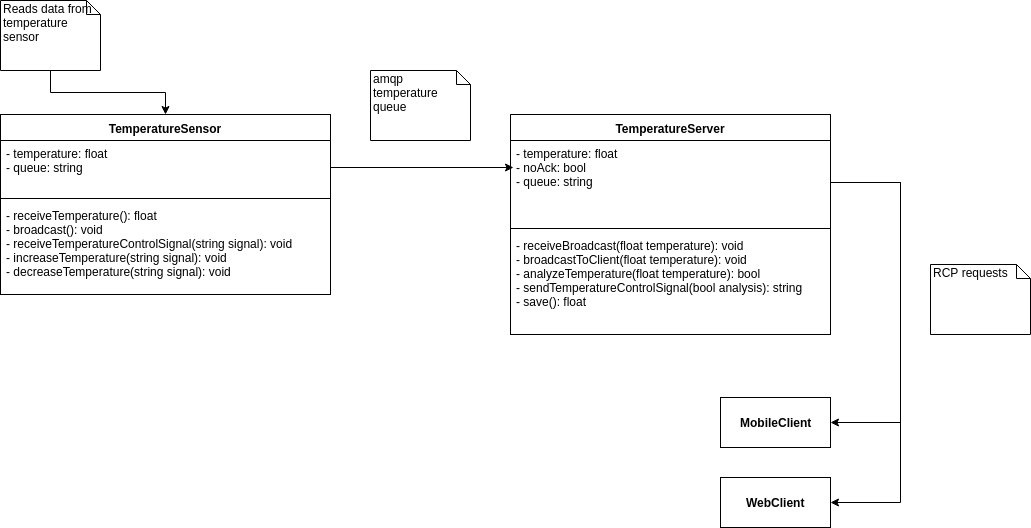
\includegraphics[width=17cm]{figuras/microservico_temperatura.png}
	\caption{Diagrama de classe do microsserviço de controle de temperatura ambiente} \label{microservico_temperatura}
\end{figure}

\subsubsection{Microsserviço de gerenciamento do usuário}

Logo abaixo, há uma ilustração da estrutura das classes que contam com o microsserviço de gerenciamento do usuário:

\begin{figure}[H]
	\centering
	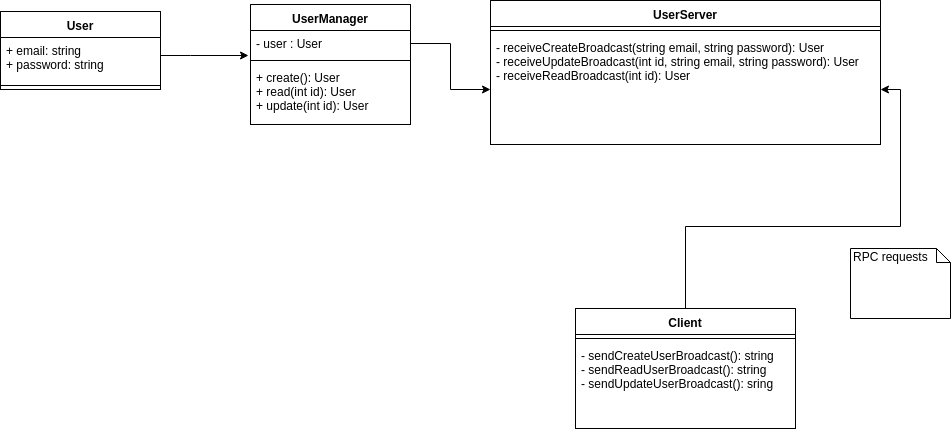
\includegraphics[width=17cm]{figuras/microservico_usuario.png}
	\caption{Diagrama de classe do microsserviço de gerenciamento do usuário} \label{microservico_usuario}
\end{figure}

Para o microsserviço de Login de usuário, o diagrama seguirá a mesma estrutura do diagrama acima.

\subsection{Diagrama de Sequência}

Diagramas de sequência podem ser utilizados para visualizar e avaliar o fluxo lógico de um sistema. Eles exibem a forma pela qual informações, ações e eventos são transmitidos entre todas as entidades relacionadas a uma funcionalidade específica.

A seguir, são apresentados os diagramas de sequência de algumas das funcionalidades chave do projeto Greenhouse.

\subsubsection{Ajuste de Temperatura Manual}

O fluxo do diagrama de sequência abaixo mostra as ações efetuadas tanto pelo usuário quanto pelos sistemas para realizar o ajuste manual da temperatura.

\begin{figure}[H]
	\centering
	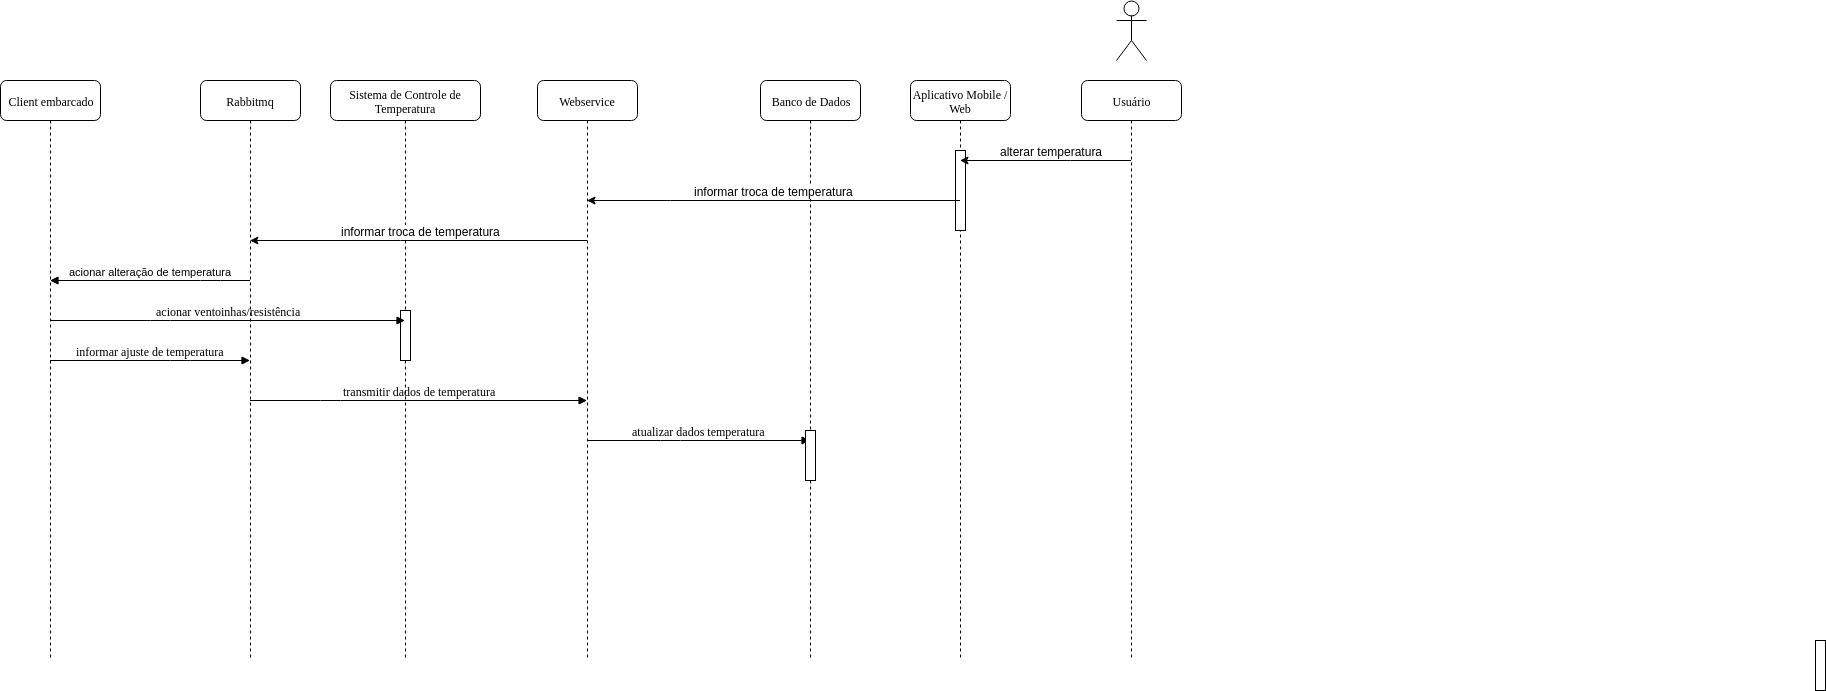
\includegraphics[width=28cm]{figuras/ajuste_manual.png}
	\caption{Diagrama de sequência do ajuste de temperatura manual} \label{ajuste_manual}
\end{figure}

\subsubsection{Ajuste de Temperatura Automático}

O fluxo do diagrama de sequência abaixo mostra as ações efetuadas tanto pelo usuário quanto pelos sistemas para realizar o ajuste automático da temperatura.

\begin{figure}[H]
	\centering
	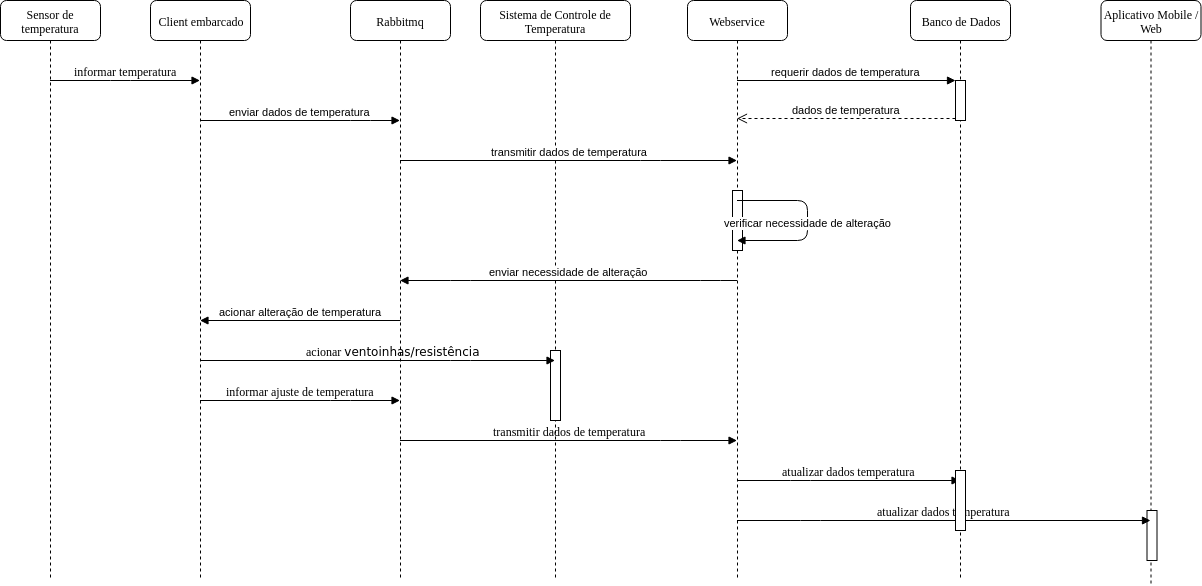
\includegraphics[width=16cm]{figuras/ajuste_automatico.png}
	\caption{Diagrama de sequência do ajuste de temperatura automático} \label{ajuste_automatico}
\end{figure}

\subsubsection{CRUD Hortaliças}

O fluxo do diagrama de sequência abaixo mostra as ações efetuadas tanto pelo usuário quanto pelos sistemas para realizar as ações presentes de criar, alterar ou deletar informações de hortaliças no banco de dados.

\begin{figure}[H]
	\centering
	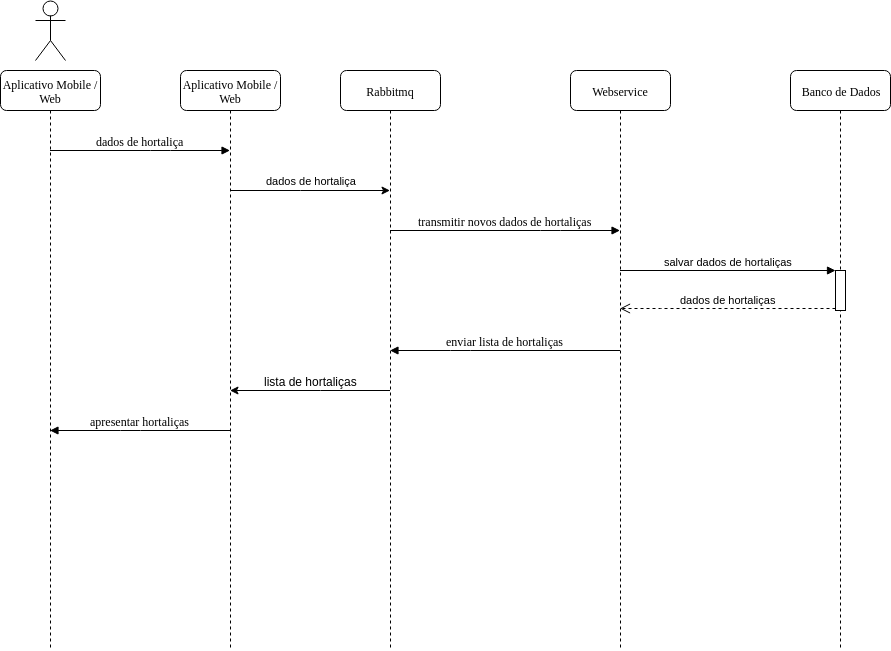
\includegraphics[width=18cm]{figuras/crud_hortalicas.png}
	\caption{Diagrama de sequência do CRUD Hortaliças} \label{crud_hortalicas}
\end{figure}

\subsubsection{Ajuste de Iluminação}

O fluxo do diagrama de sequência abaixo mostra as ações efetuadas pelos sistemas para realizar o ajuste automático de iluminação.

\begin{figure}[H]
	\centering
		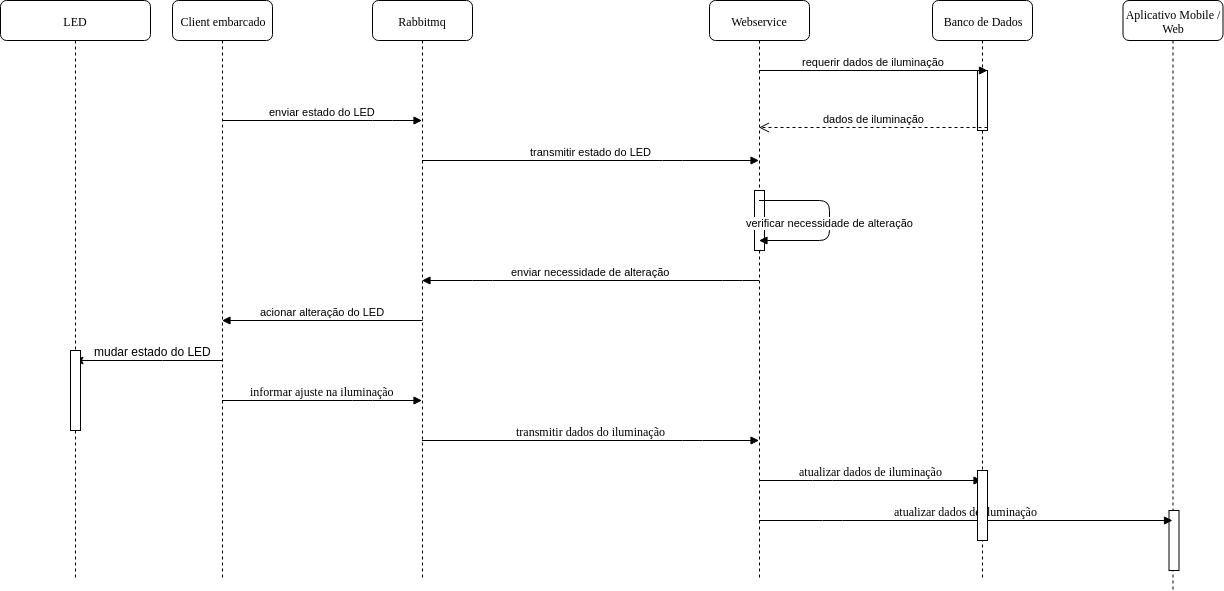
\includegraphics[width=16cm]{figuras/ajuste_iluminacao.png}
	\caption{Diagrama de sequência do ajuste de iluminação} \label{ajuste_iluminacao}
\end{figure}

\subsubsection{Editar Usuário}

O fluxo do diagrama de sequência abaixo mostra as ações efetuadas tanto pelo usuário quanto pelos sistemas para realizar a edição de um usuário no banco de dados.

\begin{figure}[H]
	\centering
	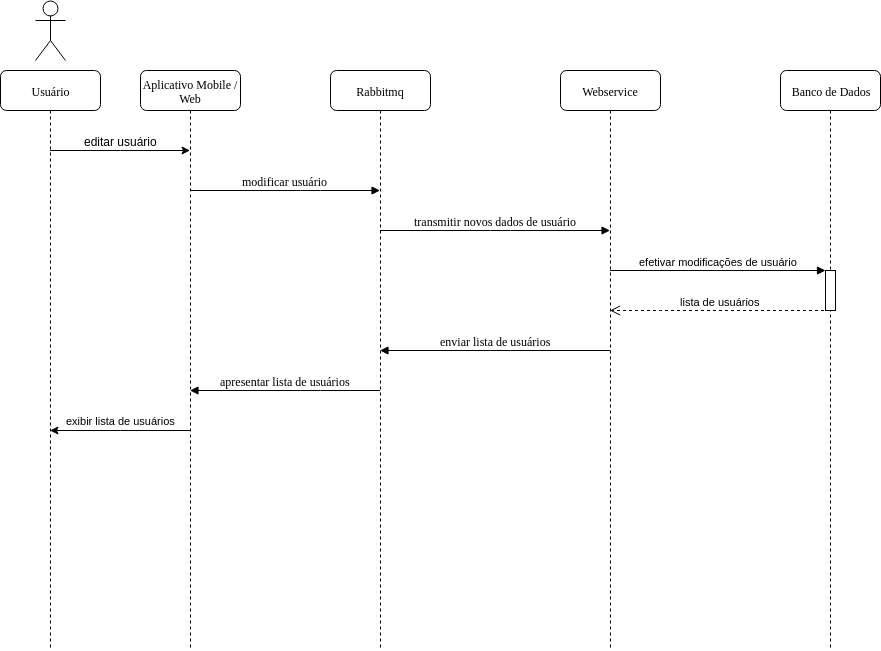
\includegraphics[width=18cm]{figuras/edicao_usuario.png}
	\caption{Diagrama de sequência de edição de usuário} \label{edicao_usuario}
\end{figure}

\subsubsection{Enviar Alerta}

O fluxo do diagrama de sequência abaixo mostra as ações efetuadas pelos sistemas para realizar o envio de alertas ao usuário.

\begin{figure}[H]
	\centering
	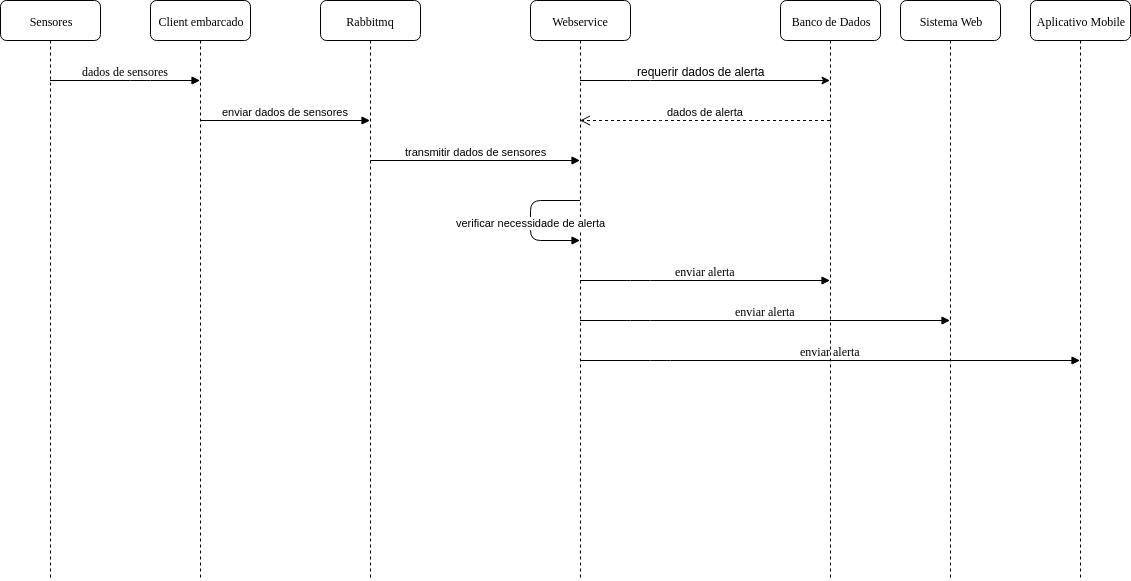
\includegraphics[width=17cm]{figuras/enviar_alerta.png}
	\caption{Diagrama de sequência de enviar alerta} \label{enviar_alerta}
\end{figure}

\subsubsection{Exibir Relatório}

O fluxo do diagrama de sequência abaixo mostra as ações efetuadas tanto pelos sistemas para exibir o relatório das informações do ambiente da estufa (i.e. média de temperatura, umidade, iluminação, e volume de água utilizado) ao usuário.

\begin{figure}[H]
	\centering
	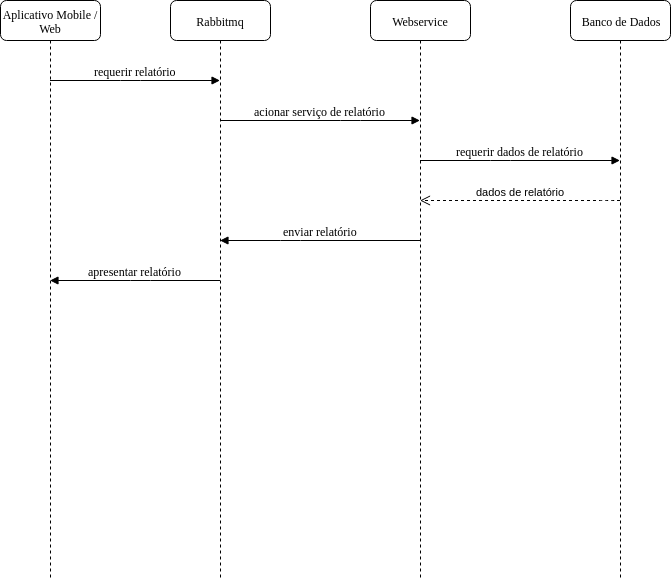
\includegraphics[width=18cm]{figuras/exibir_relatorio.png}
	\caption{Diagrama de sequência de exibir relatório} \label{exibir_relatorio}
\end{figure}

\subsubsection{Troca de Água Automática}

O fluxo do diagrama de sequência abaixo mostra as ações efetuadas pelos sistemas para realizar a troca automática de água.

\begin{figure}[H]
	\centering
	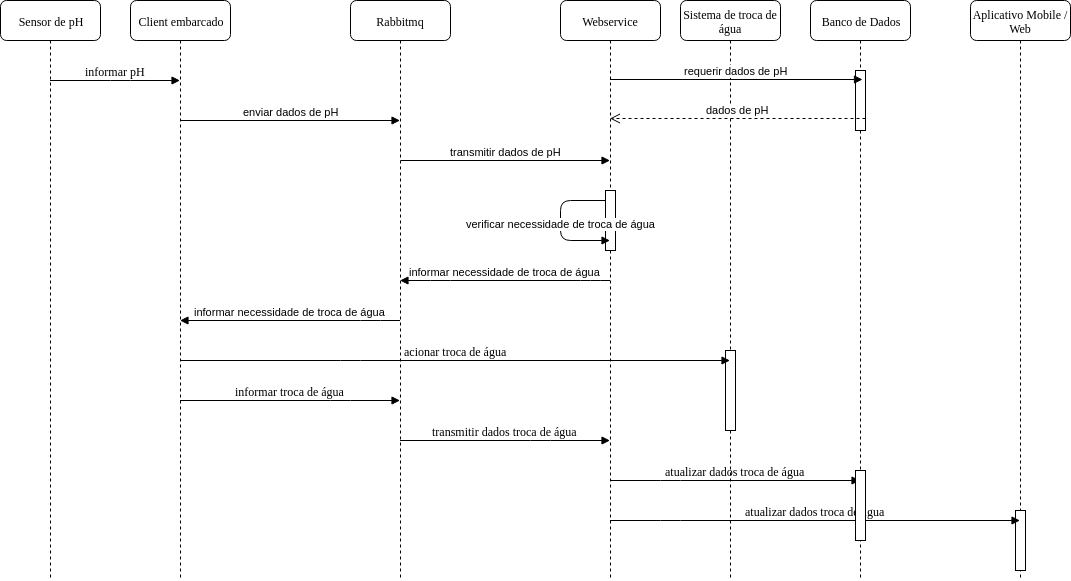
\includegraphics[width=17cm]{figuras/troca_agua.png}
	\caption{Diagrama de sequência de troca de água automática} \label{troca_agua}
\end{figure}

\subsubsection{Troca de Água Manual}

O fluxo do diagrama de sequência abaixo mostra as ações efetuadas pelos sistemas para realizar a troca manual de água.

\begin{figure}[H]
	\centering
	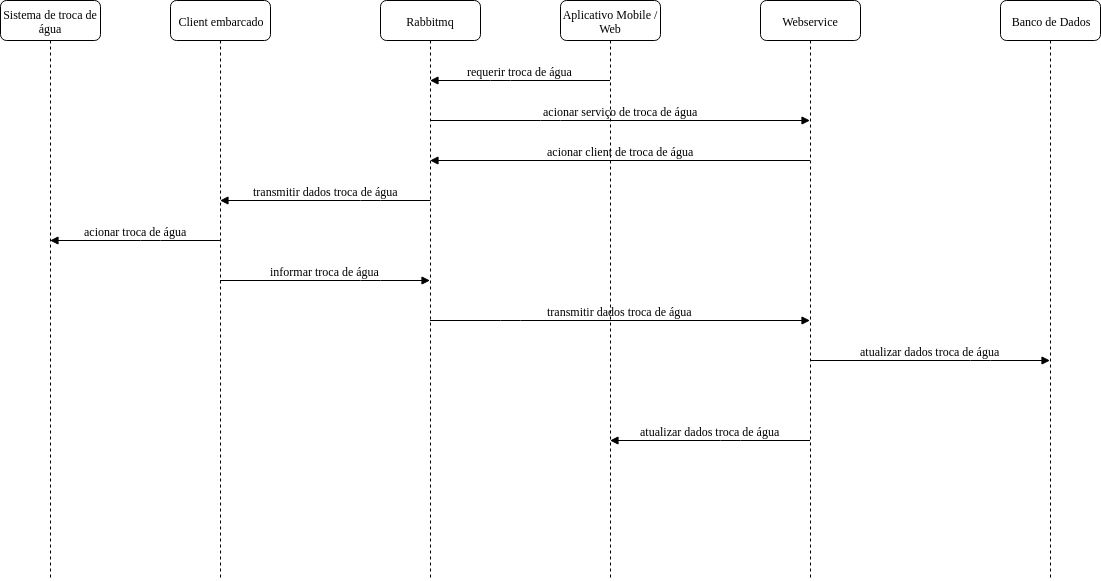
\includegraphics[width=18cm]{figuras/troca_agua_manual.png}
	\caption{Diagrama de sequência de troca de água manual} \label{troca_agua_manual}
\end{figure}